\documentclass{standalone}
\usepackage{tikz}
\usetikzlibrary{patterns, positioning}

\begin{document}
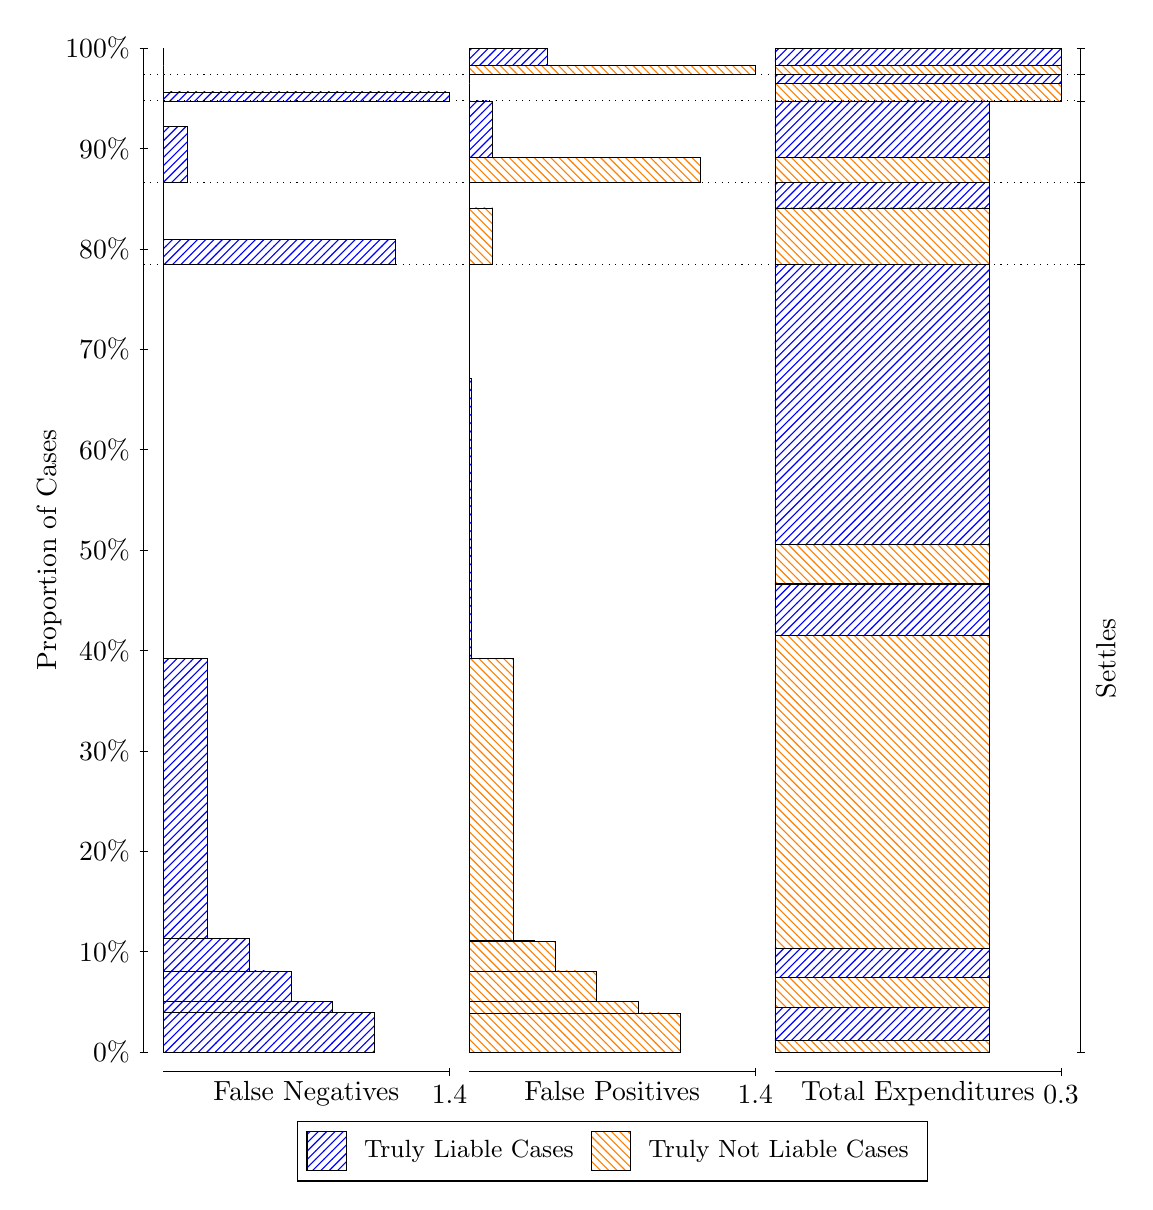
\begin{tikzpicture}
\draw[black, very thin] (1.5,1.75) -- (1.5,14.5);
\node[rotate=90, anchor=center] at (0.3, 8.125) {Proportion of Cases};
\draw[black, very thin] (1.45,1.75) -- (1.55,1.75);
\node[anchor=east] at (1.45, 1.75) {0\%};
\draw[black, very thin] (1.45,3.025) -- (1.55,3.025);
\node[anchor=east] at (1.45, 3.025) {10\%};
\draw[black, very thin] (1.45,4.3) -- (1.55,4.3);
\node[anchor=east] at (1.45, 4.3) {20\%};
\draw[black, very thin] (1.45,5.575) -- (1.55,5.575);
\node[anchor=east] at (1.45, 5.575) {30\%};
\draw[black, very thin] (1.45,6.85) -- (1.55,6.85);
\node[anchor=east] at (1.45, 6.85) {40\%};
\draw[black, very thin] (1.45,8.125) -- (1.55,8.125);
\node[anchor=east] at (1.45, 8.125) {50\%};
\draw[black, very thin] (1.45,9.4) -- (1.55,9.4);
\node[anchor=east] at (1.45, 9.4) {60\%};
\draw[black, very thin] (1.45,10.675) -- (1.55,10.675);
\node[anchor=east] at (1.45, 10.675) {70\%};
\draw[black, very thin] (1.45,11.95) -- (1.55,11.95);
\node[anchor=east] at (1.45, 11.95) {80\%};
\draw[black, very thin] (1.45,13.225) -- (1.55,13.225);
\node[anchor=east] at (1.45, 13.225) {90\%};
\draw[black, very thin] (1.45,14.5) -- (1.55,14.5);
\node[anchor=east] at (1.45, 14.5) {100\%};

\draw[black, very thin] (13.4,1.75) -- (13.4,14.5);
\draw[black, very thin] (13.35,1.75) -- (13.45,1.75);
\node[anchor=west] at (13.35, 1.75) {};
\draw[black, very thin] (13.35,11.75) -- (13.45,11.75);
\node[anchor=west] at (13.35, 11.75) {};
\draw[black, very thin] (13.35,12.792) -- (13.45,12.792);
\node[anchor=west] at (13.35, 12.792) {};
\draw[black, very thin] (13.35,13.83) -- (13.45,13.83);
\node[anchor=west] at (13.35, 13.83) {};
\draw[black, very thin] (13.35,14.164) -- (13.45,14.164);
\node[anchor=west] at (13.35, 14.164) {};
\draw[black, very thin] (13.35,14.5) -- (13.45,14.5);
\node[anchor=west] at (13.35, 14.5) {};

\draw[black, very thin, pattern color=blue, pattern=north east lines] (1.75,1.75) rectangle (4.4255,2.2547);
\draw[black, very thin, pattern color=blue, pattern=north east lines] (1.75,2.2547) rectangle (4.1612,2.2567);
\draw[black, very thin, pattern color=blue, pattern=north east lines] (1.75,2.2567) rectangle (3.897,2.3935);
\draw[black, very thin, pattern color=blue, pattern=north east lines] (1.75,2.3935) rectangle (3.6327,2.3958);
\draw[black, very thin, pattern color=blue, pattern=north east lines] (1.75,2.3958) rectangle (3.6327,2.3973);
\draw[black, very thin, pattern color=blue, pattern=north east lines] (1.75,2.3973) rectangle (3.3685,2.7718);
\draw[black, very thin, pattern color=blue, pattern=north east lines] (1.75,2.7718) rectangle (3.1042,2.7792);
\draw[black, very thin, pattern color=blue, pattern=north east lines] (1.75,2.7792) rectangle (2.84,3.1901);
\draw[black, very thin, pattern color=blue, pattern=north east lines] (1.75,3.1901) rectangle (2.5758,3.1969);
\draw[black, very thin, pattern color=blue, pattern=north east lines] (1.75,3.1969) rectangle (2.3115,6.7498);
\draw[black, very thin, pattern color=orange, pattern=north west lines] (1.75,6.7498) rectangle (1.75,11.75);
\draw[black, very thin, pattern color=blue, pattern=north east lines] (1.75,11.75) rectangle (4.6897,12.072);
\draw[black, very thin, pattern color=orange, pattern=north west lines] (1.75,12.072) rectangle (1.75,12.792);
\draw[black, very thin, pattern color=blue, pattern=north east lines] (1.75,12.792) rectangle (2.0473,13.509);
\draw[black, very thin, pattern color=orange, pattern=north west lines] (1.75,13.509) rectangle (1.75,13.83);
\draw[black, very thin, pattern color=blue, pattern=north east lines] (1.75,13.83) rectangle (5.3833,13.942);
\draw[black, very thin, pattern color=orange, pattern=north west lines] (1.75,13.942) rectangle (1.75,14.164);
\draw[black, very thin, pattern color=orange, pattern=north west lines] (1.75,14.164) rectangle (1.75,14.276);
\draw[black, very thin, pattern color=blue, pattern=north east lines] (1.75,14.276) rectangle (1.75,14.5);
\draw[black, very thin, pattern color=orange, pattern=north west lines] (5.6333,1.75) rectangle (8.3088,2.2427);
\draw[black, very thin, pattern color=orange, pattern=north west lines] (5.6333,2.2427) rectangle (8.0445,2.2452);
\draw[black, very thin, pattern color=orange, pattern=north west lines] (5.6333,2.2452) rectangle (7.7803,2.3932);
\draw[black, very thin, pattern color=orange, pattern=north west lines] (5.6333,2.3932) rectangle (7.5161,2.397);
\draw[black, very thin, pattern color=orange, pattern=north west lines] (5.6333,2.397) rectangle (7.2518,2.7712);
\draw[black, very thin, pattern color=orange, pattern=north west lines] (5.6333,2.7712) rectangle (6.9876,2.779);
\draw[black, very thin, pattern color=orange, pattern=north west lines] (5.6333,2.779) rectangle (6.7233,3.1587);
\draw[black, very thin, pattern color=orange, pattern=north west lines] (5.6333,3.1587) rectangle (6.4591,3.1643);
\draw[black, very thin, pattern color=orange, pattern=north west lines] (5.6333,3.1643) rectangle (6.1948,6.7502);
\draw[black, very thin, pattern color=blue, pattern=north east lines] (5.6333,6.7502) rectangle (5.6664,10.303);
\draw[black, very thin, pattern color=blue, pattern=north east lines] (5.6333,10.303) rectangle (5.6333,11.75);
\draw[black, very thin, pattern color=orange, pattern=north west lines] (5.6333,11.75) rectangle (5.9306,12.47);
\draw[black, very thin, pattern color=blue, pattern=north east lines] (5.6333,12.47) rectangle (5.6333,12.792);
\draw[black, very thin, pattern color=orange, pattern=north west lines] (5.6333,12.792) rectangle (8.573,13.112);
\draw[black, very thin, pattern color=blue, pattern=north east lines] (5.6333,13.112) rectangle (5.9306,13.83);
\draw[black, very thin, pattern color=orange, pattern=north west lines] (5.6333,13.83) rectangle (5.6333,14.052);
\draw[black, very thin, pattern color=blue, pattern=north east lines] (5.6333,14.052) rectangle (5.6333,14.164);
\draw[black, very thin, pattern color=orange, pattern=north west lines] (5.6333,14.164) rectangle (9.2667,14.276);
\draw[black, very thin, pattern color=blue, pattern=north east lines] (5.6333,14.276) rectangle (6.6242,14.5);
\draw[black, very thin, pattern color=orange, pattern=north west lines] (9.5167,1.75) rectangle (12.242,1.9004);
\draw[black, very thin, pattern color=blue, pattern=north east lines] (9.5167,1.9004) rectangle (12.242,2.3181);
\draw[black, very thin, pattern color=orange, pattern=north west lines] (9.5167,2.3181) rectangle (12.242,2.6924);
\draw[black, very thin, pattern color=blue, pattern=north east lines] (9.5167,2.6924) rectangle (12.242,3.067);
\draw[black, very thin, pattern color=orange, pattern=north west lines] (9.5167,3.067) rectangle (12.242,7.0446);
\draw[black, very thin, pattern color=blue, pattern=north east lines] (9.5167,7.0446) rectangle (12.242,7.6904);
\draw[black, very thin, pattern color=orange, pattern=north west lines] (9.5167,7.6904) rectangle (12.242,7.6956);
\draw[black, very thin, pattern color=blue, pattern=north east lines] (9.5167,7.6956) rectangle (12.242,7.7044);
\draw[black, very thin, pattern color=orange, pattern=north west lines] (9.5167,7.7044) rectangle (12.242,8.1971);
\draw[black, very thin, pattern color=blue, pattern=north east lines] (9.5167,8.1971) rectangle (12.242,11.75);
\draw[black, very thin, pattern color=orange, pattern=north west lines] (9.5167,11.75) rectangle (12.242,12.47);
\draw[black, very thin, pattern color=blue, pattern=north east lines] (9.5167,12.47) rectangle (12.242,12.792);
\draw[black, very thin, pattern color=orange, pattern=north west lines] (9.5167,12.792) rectangle (12.242,13.112);
\draw[black, very thin, pattern color=blue, pattern=north east lines] (9.5167,13.112) rectangle (12.242,13.83);
\draw[black, very thin, pattern color=orange, pattern=north west lines] (9.5167,13.83) rectangle (13.15,14.052);
\draw[black, very thin, pattern color=blue, pattern=north east lines] (9.5167,14.052) rectangle (13.15,14.164);
\draw[black, very thin, pattern color=orange, pattern=north west lines] (9.5167,14.164) rectangle (13.15,14.276);
\draw[black, very thin, pattern color=blue, pattern=north east lines] (9.5167,14.276) rectangle (13.15,14.5);
\draw[black, dotted] (1.5,11.75) -- (13.4,11.75);
\draw[black, dotted] (1.5,12.792) -- (13.4,12.792);
\draw[black, dotted] (1.5,13.83) -- (13.4,13.83);
\draw[black, dotted] (1.5,14.164) -- (13.4,14.164);
\draw[black, very thin] (1.75,1.5) -- (5.3833,1.5);
\node[anchor=north] at (3.5667, 1.5) {False Negatives};
\draw[black, very thin] (5.3833,1.45) -- (5.3833,1.55);
\node[anchor=north] at (5.3833, 1.45) {1.4};

\draw[black, very thin] (5.6333,1.5) -- (9.2667,1.5);
\node[anchor=north] at (7.45, 1.5) {False Positives};
\draw[black, very thin] (9.2667,1.45) -- (9.2667,1.55);
\node[anchor=north] at (9.2667, 1.45) {1.4};

\draw[black, very thin] (9.5167,1.5) -- (13.15,1.5);
\node[anchor=north] at (11.333, 1.5) {Total Expenditures};
\draw[black, very thin] (13.15,1.45) -- (13.15,1.55);
\node[anchor=north] at (13.15, 1.45) {0.3};

\node[black, centered, rotate=90] at (13.72, 6.75) {Settles};





\draw (7.449999999999999,1.5) node[draw=none] (baseCoordinate) {};
\begin{scope}[align=center]
        \matrix[scale=0.5, draw=black, below=0.5cm of baseCoordinate, nodes={draw}, column sep=0.1cm]{
            \node[rectangle, draw, minimum width=0.5cm, minimum height=0.5cm, pattern=north east lines, pattern color=blue] {}; &
            \node[draw=none, font=\small] (B) {Truly Liable Cases}; &
            \node[rectangle, draw, minimum width=0.5cm, minimum height=0.5cm, pattern=north west lines, pattern color=orange] {}; &
            \node[draw=none, font=\small] (B) {Truly Not Liable Cases}; \\
            };
\end{scope}

\end{tikzpicture}
\end{document}